\documentclass[11pt,a4paper]{article}
\usepackage{fontspec}
\setmainfont{TeX Gyre Pagella}
\newfontfamily\headfont{Inter}[UprightFont=*-ExtraBold,BoldFont=*-ExtraBold,Extension=.otf,Path=/usr/share/fonts/opentype/inter/]
\usepackage[a4paper,margin=2.3cm]{geometry}
\usepackage{graphicx,booktabs,float,caption,array,xcolor,longtable}
\usepackage{xurl}
\usepackage[hidelinks]{hyperref}
\usepackage{titlesec}
\usepackage[round]{natbib}
\usepackage{setspace}
\setstretch{1.05}
\renewcommand{\topfraction}{0.9}
\renewcommand{\bottomfraction}{0.8}
\renewcommand{\textfraction}{0.1}
\renewcommand{\floatpagefraction}{0.75}
\setlength{\parindent}{0pt}
\setlength{\parskip}{0.55em}
\titleformat{\section}{\headfont\Large}{\thesection}{0.8em}{}
\titleformat{\subsection}{\headfont\large}{\thesubsection}{0.8em}{}
\captionsetup{font=small,labelfont=bf}
\urlstyle{same}
\hypersetup{pdftitle={Shipwrecks of the World, and How Many over Time},pdfauthor={Tristan Hotham}}

\begin{document}
\begin{center}
{\Large\bfseries Shipwrecks of the World, and How Many over Time\par}
\vspace{0.4em}
{\large Three centuries of recorded losses:\\243,071 wrecks in Wikipedia's lists of shipwrecks, 1700 to 2025\par}
\vspace{1.2em}
{\large Tristan Hotham\par}
\vspace{0.3em}
{\small Independent researcher\\
ORCID: 0000-0003-4931-9349\\
DOI: https://doi.org/10.5281/zenodo.23850289\par}
\vspace{0.8em}
2026
\end{center}

\begin{quote}
\small
\begin{center}\textbf{Abstract}\end{center}
English Wikipedia lists shipwrecks month by month from the 1820s and year by year or decade by decade before that. I turned every list from 1700 to 2025 into one table of 243,071 wrecks, after removing 9,217 duplicates, and counted them by year, cause and flag. Three of the five worst years are war years: 1944 (4,570 wrecks), 1917 (4,083) and 1942 (4,027). The Second World War averages 3,044 listed wrecks a year, 6.9 times the interwar rate, and 69\% of its entries were lost to torpedoes, aircraft, mines or gunfire. But the series is shaped as much by its sources as by the sea: 71\% of all entries are from the 1800s, when the lists average 2,746 wrecks a year from 1850 to 1879, and 66\% of those are British ships, reflecting the British newspapers and Lloyd's List from which the pages were compiled; between 1890 and 1913 the average falls to 483. Most nineteenth-century losses were strandings (65\%). I pair the series with a map of 52,124 wrecks with coordinates from the lists, Wikidata (including bulk imports from the Scottish and Welsh heritage records) and NOAA's wreck charts, which has its own strong bias: 61\% of mapped wrecks lie in UK waters. Both are records of recording as much as of loss.

\textbf{Keywords:} shipwrecks; maritime history; Wikipedia; Lloyd's List; World War; Wikidata; AWOIS; sampling bias; open data; mapping
\end{quote}

\section{Introduction}
How many ships have been lost at sea, and when? UNESCO's frequently quoted estimate is that some three million wrecks lie on the sea bed \citep{unesco}, but no census exists. What exists are records: newspaper casualty columns, insurers' lists, naval loss returns, hydrographic charts and heritage registers. Each counts what its compilers could see.

English Wikipedia contains an extraordinary compilation of such records. Volunteers have built a ``List of shipwrecks'' page for every month since the 1820s, and for every year or decade before, each entry giving a date, the ship, its flag and a short description of the loss, usually with a citation \citep{wikilists}. This paper turns those pages into a single time series from 1700 to 2025, by cause and by flag, and asks what it shows and what it cannot. It adds a map of every wreck I could find in open data with coordinates, and an interactive version with a year slider (\url{https://maps.tristanhotham.com/world-shipwrecks/}).

\section{Data}
\textbf{Wikipedia lists.} A structured table was scraped from every English Wikipedia ``List of shipwrecks'' page for 1700 to 2025: the decade pages for the 1700s to 1750s, year pages, and monthly pages from 1820 (year pages for those years hold only entries of unknown date). It has 252,288 rows with page title, year, month, date heading, ship, flag, a cause sorted into buckets (wrecked or aground, foundered, collision, fire or explosion, torpedo, mine, aircraft, other war, scuttled, other or unknown) and, for 15,524 entries, coordinates. Wikipedia text is CC BY-SA 4.0; I credit Wikipedia contributors and share the derived table under the same licence.

\textbf{Wikidata.} Every Wikidata \citep{wikidata} item with coordinates that is an instance of shipwreck (Q852190) or has a shipwrecking event, through the QLever service: 30,940 items, of which 30,821 remain after dropping 86 without usable coordinates and 33 that are not vessels. Two bulk imports dominate: Scottish records from Canmore \citep{canmore} and Welsh records from Coflein \citep{coflein}. Further Wikidata extracts give dated events (shipwrecking, sinking, scuttling, destruction) for 1,496 items and other dates.

\textbf{NOAA AWOIS.} The wrecks layer of the Automated Wreck and Obstruction Information System \citep{awois}, a public-domain record of wrecks in United States waters, from a copy on GitHub \citep{awoisgh}: 6,201 records, 6,170 after removing rocks and duplicates of Wikidata wrecks.

\textbf{Ancient wrecks and geography.} The Summary Geodatabase of Shipwrecks 1500~BCE to 1500~CE (Harvard Mapping Past Societies, after \citealt{strauss} and \citealt{parker}) via \citet{ancientgh}, used only as counts per century because its licence is not stated in that copy; Natural Earth \citep{naturalearth} outlines.

\section{Methods}
\subsection{The list series}
I removed 9,217 rows that repeat the same ship under the same date heading on the same page, keeping rows without a ship name (9,767), since several unnamed vessels can be lost on one day; 243,071 entries remain. The year comes from the page or, on the decade pages, from the date heading where it contains one; 516 entries without a year count only by decade. Causes are grouped into war (torpedo, mine, aircraft, other war), foundered or storm, wrecked or ran aground, collision, fire or explosion, scuttled, and not recorded. Flags are grouped across regimes and spellings: for example the United Kingdom of Great Britain and Ireland, the Kingdom of Great Britain and the United Kingdom as the United Kingdom; Prussia, Hamburg, the German Empire and Nazi Germany as Germany; the Russian Empire and the Soviet Union together.

\subsection{The map}
Years of loss for Wikidata wrecks come, in order, from the latest dated shipwrecking or sinking event, the point in time, service retirement, dissolution or end time, inception of an item that is only a wreck, and then text (``sank in 1901''; Canmore labels of documented losses such as ``Unknown 1830''). For AWOIS they come from dates after ``sunk'' in the survey notes or the year sunk field. I never infer a year from a launch date or a war. List entries with coordinates are mapped unless they match a Wikidata or AWOIS wreck of the same name within 20~km (391 such matches, which also gave 163 wrecks a year). Table~\ref{tab:methods} lists the sources of the 18,596 mapped years.

\begin{table}[tbp]\centering\small\caption{Where the years of loss come from (first source that applies).}\label{tab:methods}\begin{tabular}{lr}\toprule Source of the year & Wrecks\\\midrule
Wikipedia list page & 15,130\\
label: unknown vessel lost in a year (Canmore) & 1,492\\
AWOIS: year sunk in the history text & 950\\
Wikidata: date of the shipwrecking or sinking event & 568\\
AWOIS: YEARSUNK field & 179\\
Wikipedia list page (matched entry) & 163\\
Wikidata: service retirement & 46\\
text: sank or wrecked in a year & 24\\
Wikidata: dissolved or end time & 19\\
Wikidata: inception of a wreck-only item & 9\\
Wikidata: point in time & 7\\
AWOIS (record matched to a Wikidata item) & 4\\
label: year in brackets & 3\\
label: loss year after a plus sign & 2\\
\bottomrule\end{tabular}\end{table}

\section{Results}
\subsection{How many over time}
Figure~\ref{fig:years} shows the series. It rises from 8.4 entries a year before 1750 to a nineteenth-century plateau that peaks at 3,794 in 1880, averaging 2,746 a year from 1850 to 1879. It then drops sharply: from 1890 to 1913 the average is 483. The two world wars stand out. The First averages 2,064 a year, 4.3 times the years before it, with 4,083 in 1917; the Second averages 3,044, 6.9 times the 440 a year of 1919 to 1938 and 1.11 times the 1850 to 1879 average, with 4,027 in 1942 and 4,570 in 1944, the highest of any year. Since 1966 the lists hold about 137 wrecks a year. Table~\ref{tab:top} lists the ten worst years.

\begin{figure}[tbp]\centering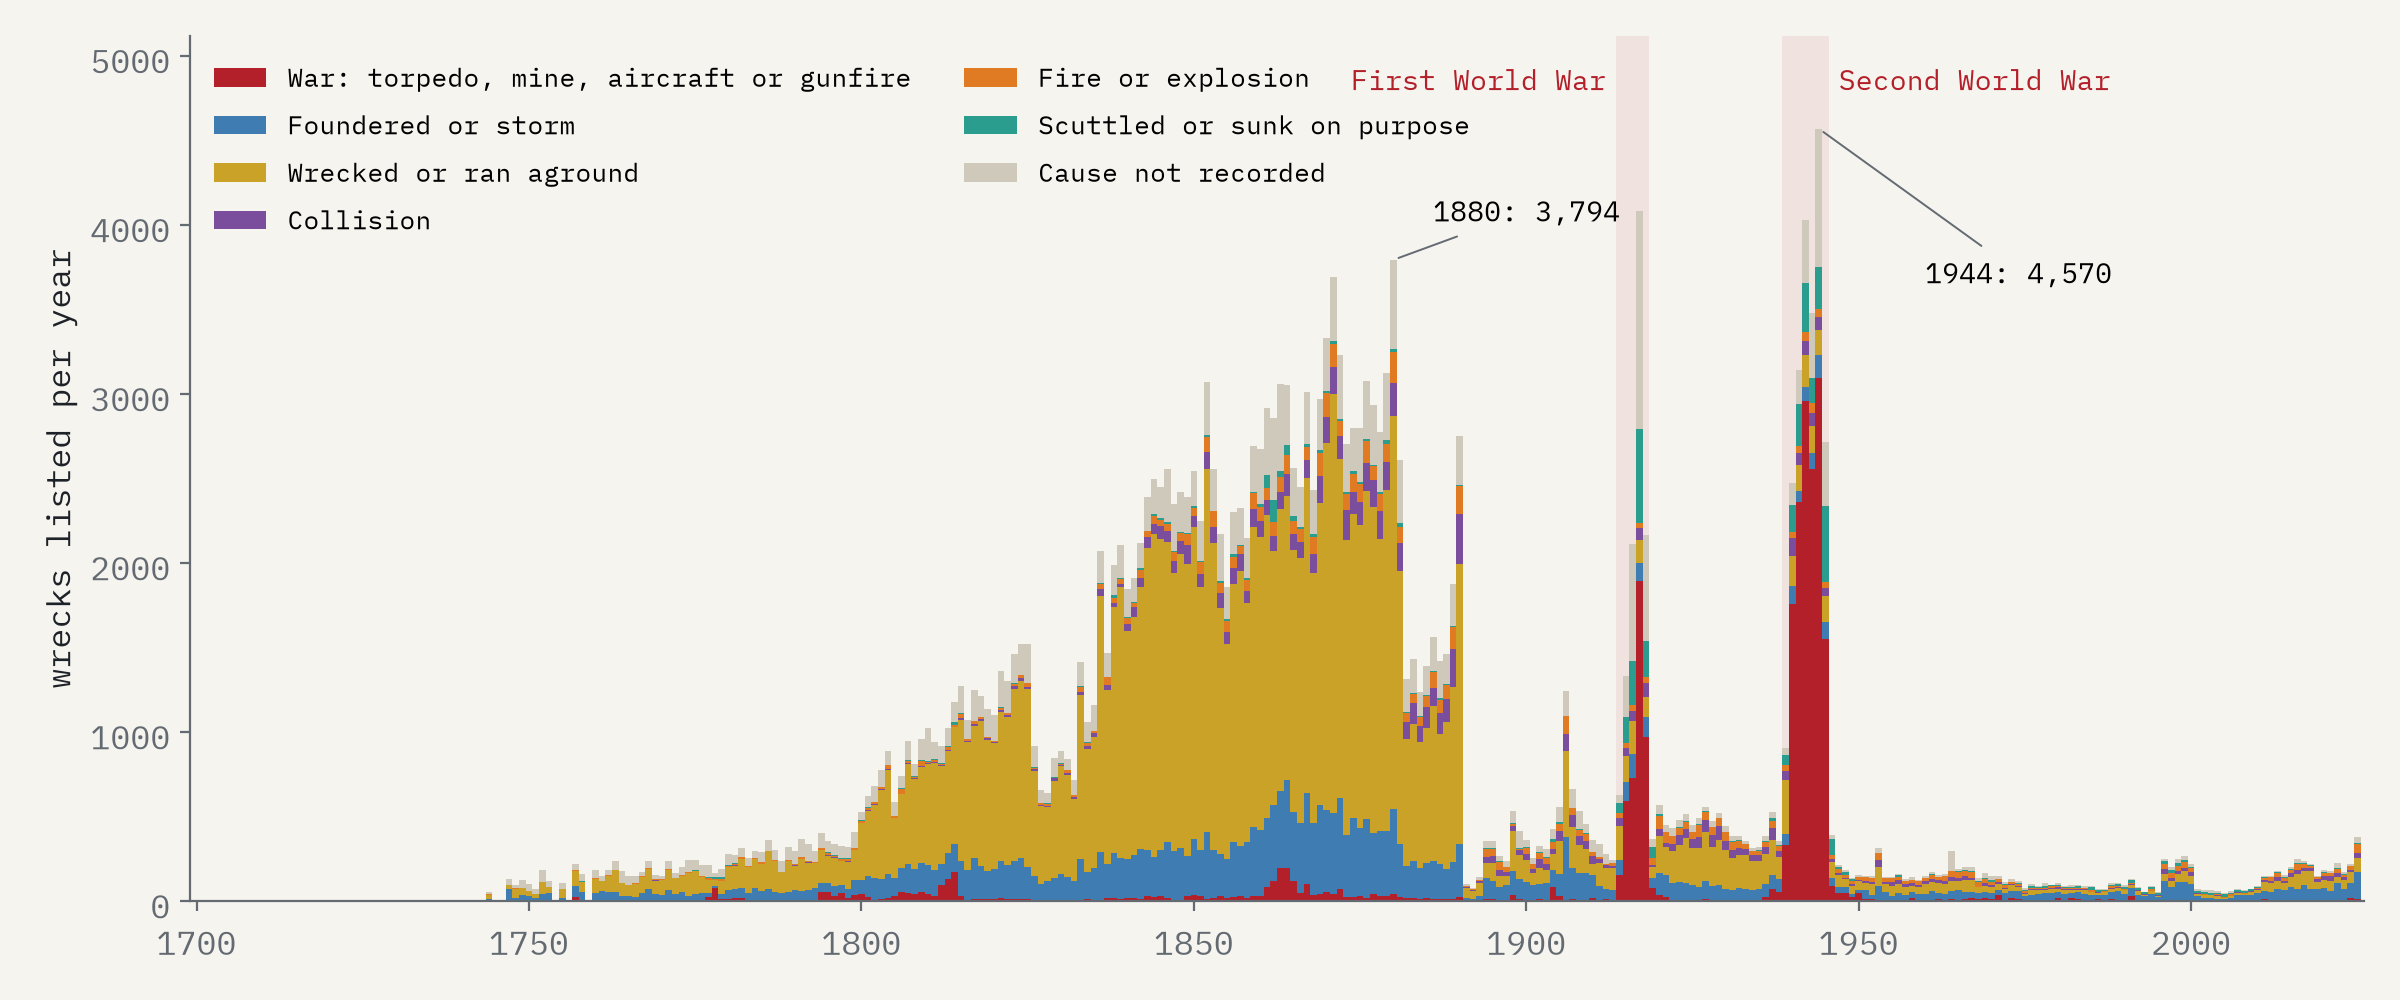
\includegraphics[width=\textwidth]{f_years.png}
\caption{Shipwrecks listed on Wikipedia per year, 1700 to 2025, by cause. Shaded: the two world wars.}\label{fig:years}\end{figure}

\begin{table}[tbp]\centering\small\caption{The ten years with most shipwrecks listed on Wikipedia.}\label{tab:top}\begin{tabular}{rr}\toprule Year & Wrecks listed\\\midrule
1944 & 4,570\\
1917 & 4,083\\
1942 & 4,027\\
1880 & 3,794\\
1871 & 3,692\\
1943 & 3,478\\
1870 & 3,329\\
1872 & 3,230\\
1941 & 3,140\\
1879 & 3,125\\
\bottomrule\end{tabular}\end{table}

\subsection{Causes}
88\% of entries have a cause (Figure~\ref{fig:causes}). Over the whole period most wrecks ran aground or were driven ashore (53\%), followed by foundering (15\%), war (10\%), collision (4\%), fire or explosion (4\%) and scuttling (2\%). In the 1800s, 65\% of entries were strandings and 14\% founderings. War causes 42\% of First World War entries and 69\% of Second World War entries, and 78\% of all war losses fall in the two wars. In the Second World War, torpedoes account for 6,588 entries, aircraft 4,345, mines 2,432 and gunfire, capture or other action 1,259.

\begin{figure}[tbp]\centering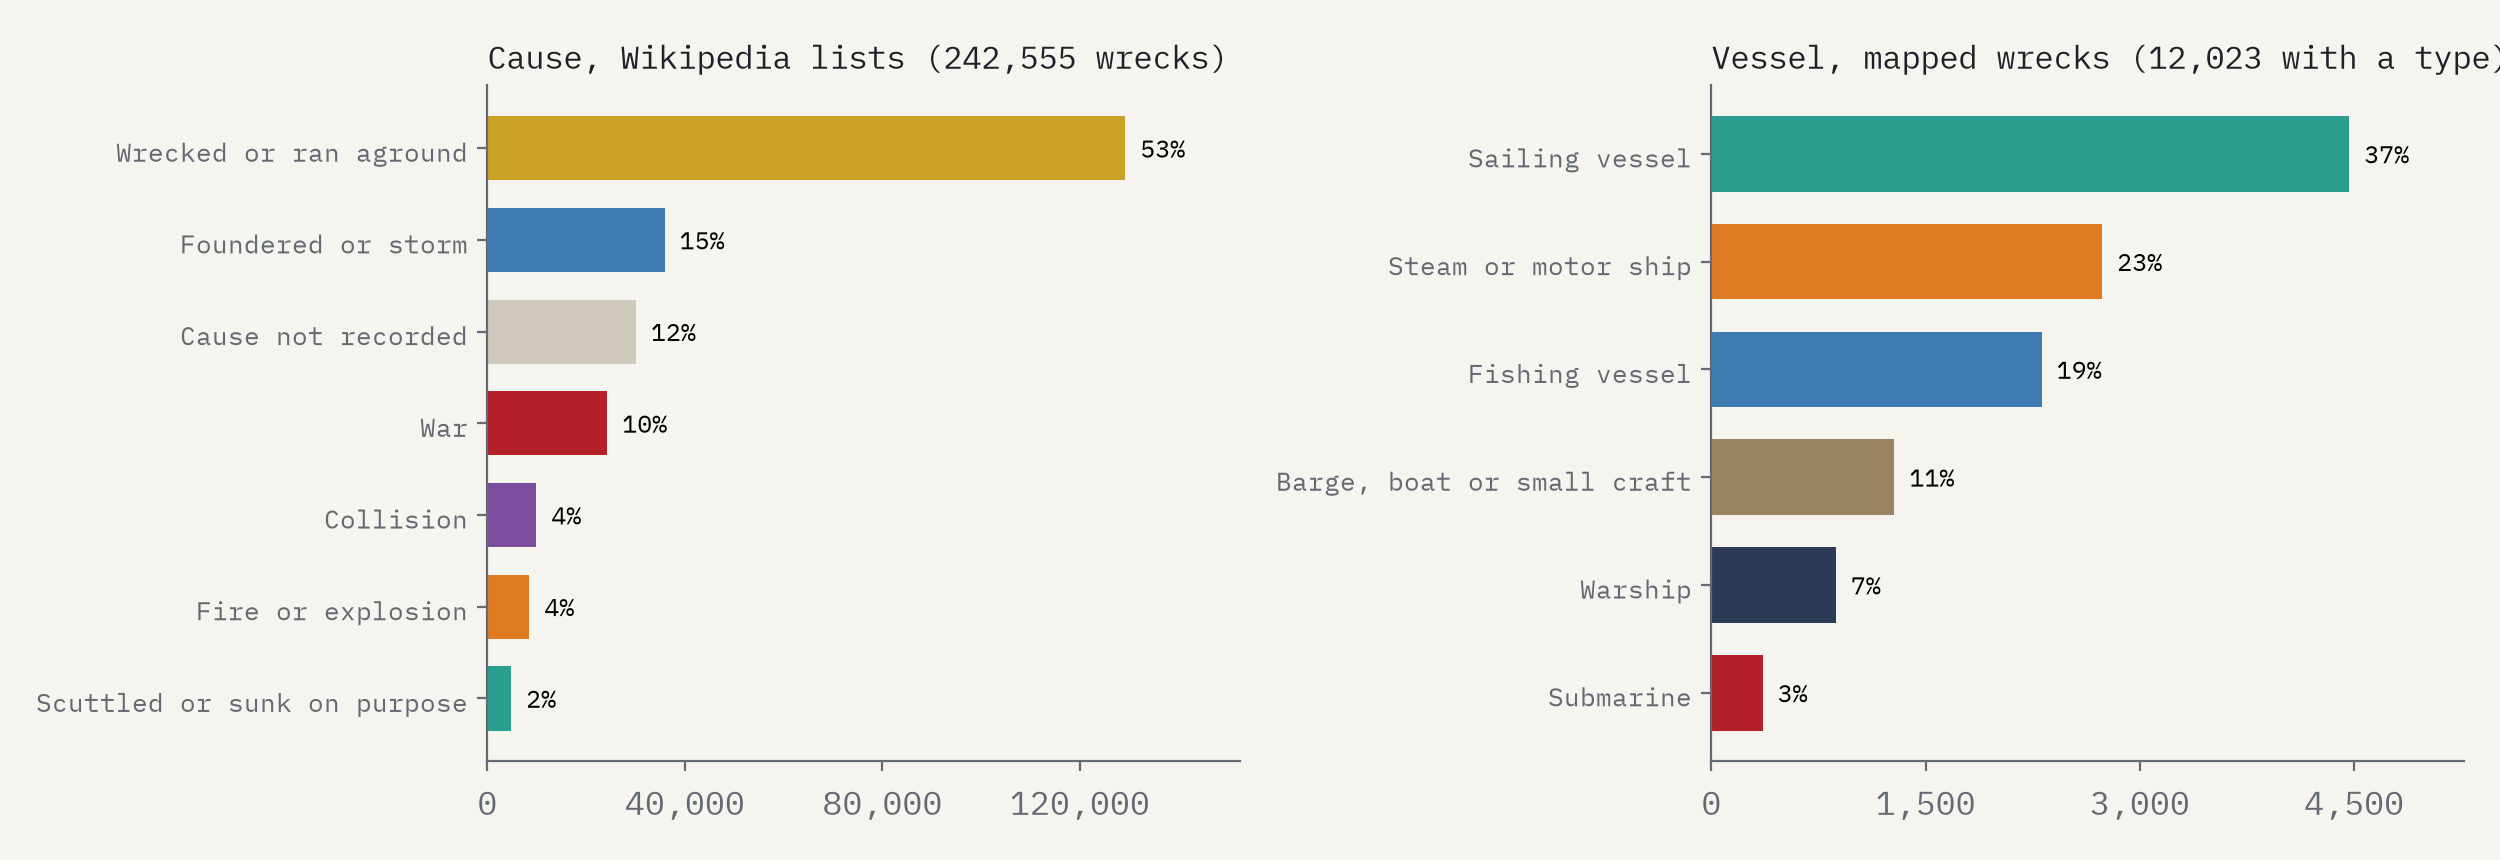
\includegraphics[width=\textwidth]{f_causes.png}
\caption{Left: causes of listed wrecks. Right: vessel types of mapped wrecks, where known.}\label{fig:causes}\end{figure}

\subsection{Flags}
93\% of entries have a flag. 56\% are British, 10.2\% American, then German, French and Norwegian (Table~\ref{tab:flags}). The British share is 66\% in the 1800s and falls to 24\% in 1939 to 1945, when German, Japanese, Italian and Soviet losses join the lists (Figure~\ref{fig:flags}).

\begin{figure}[tbp]\centering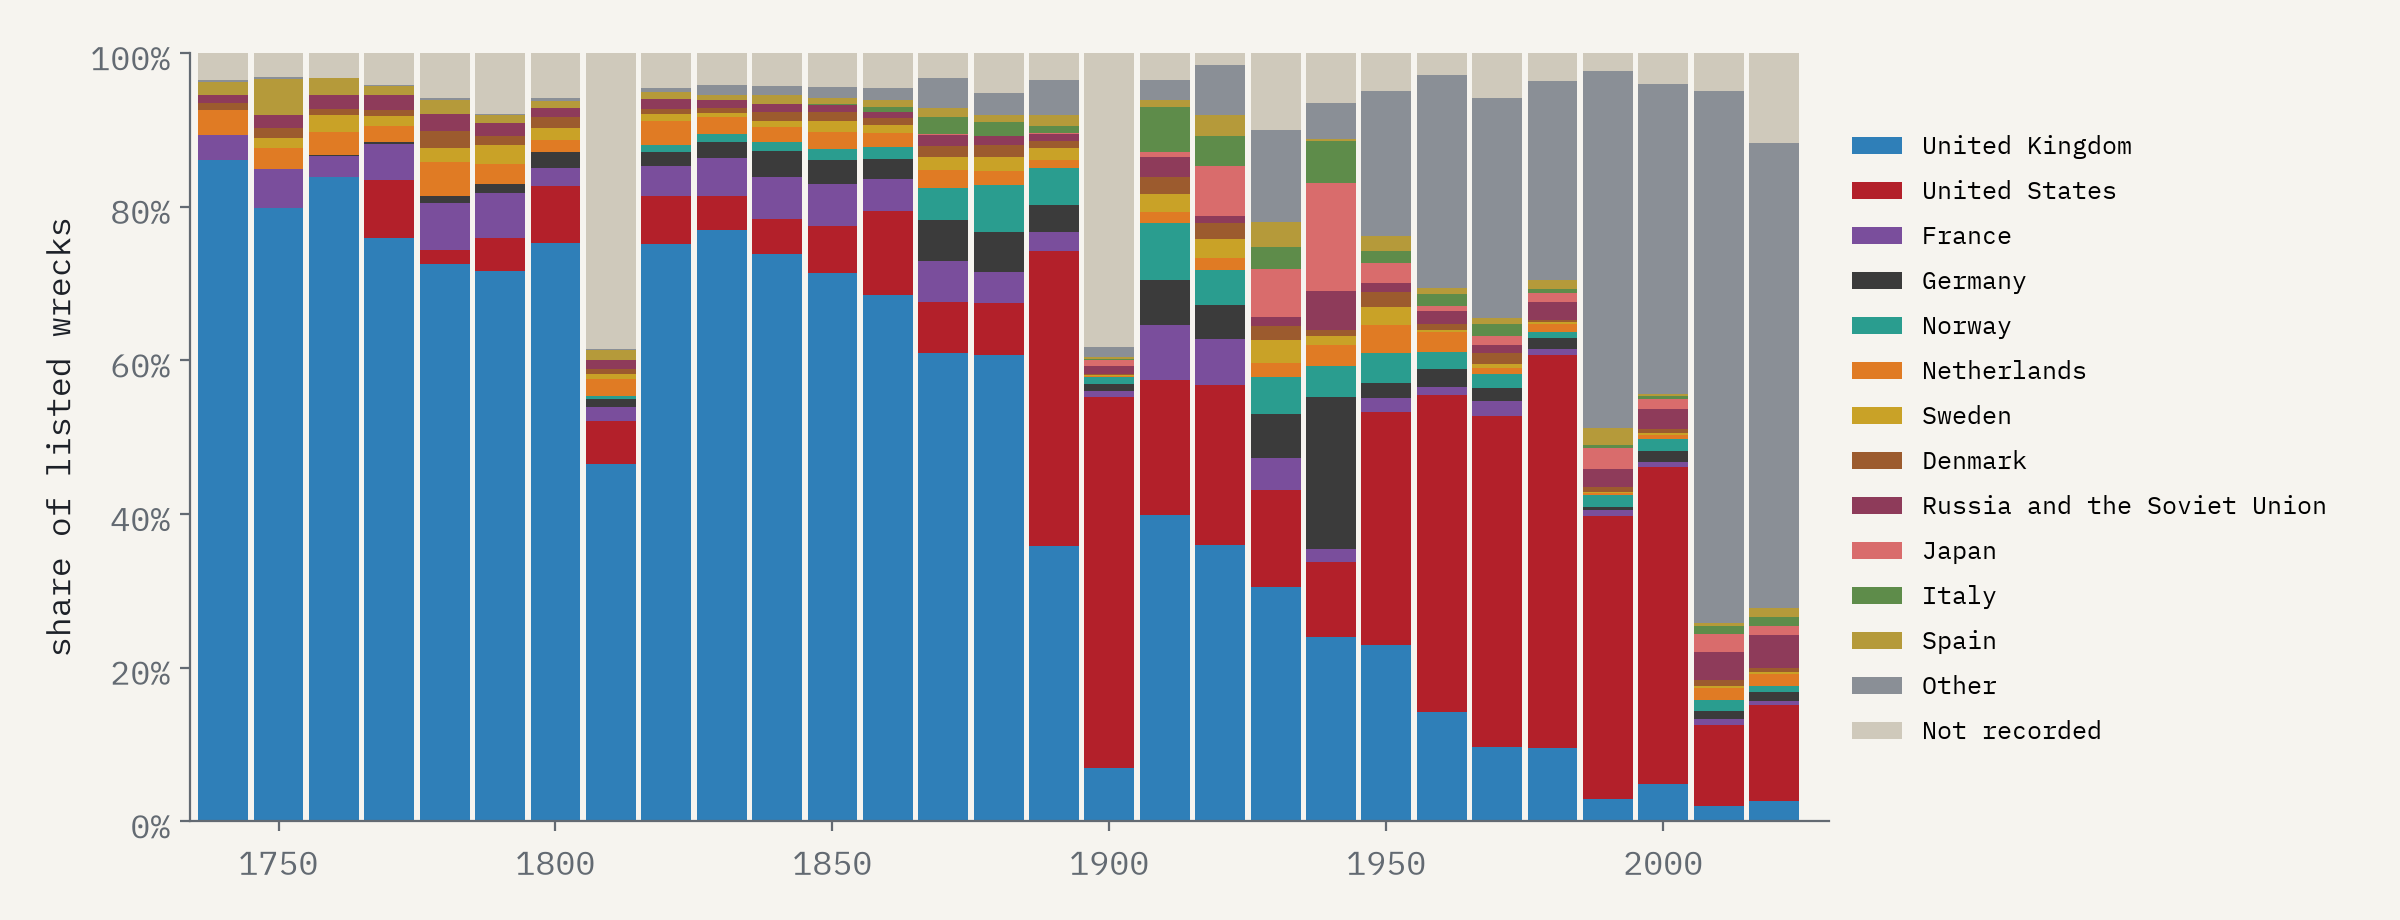
\includegraphics[width=\textwidth]{f_flags.png}
\caption{Share of listed wrecks by flag, per decade (decades with at least 300 entries).}\label{fig:flags}\end{figure}

\begin{table}[tbp]\centering\small\caption{Listed wrecks by flag group, 1700 to 2025, and in 1939 to 1945.}\label{tab:flags}\begin{tabular}{lrrr}\toprule Flag & Wrecks & Share & 1939 to 1945\\\midrule
United Kingdom & 135,453 & 55.8\% & 5,112\\
United States & 24,654 & 10.2\% & 1,752\\
Not recorded & 16,402 & 6.8\% & 1,314\\
Germany & 11,130 & 4.6\% & 4,121\\
France & 10,006 & 4.1\% & 401\\
Other & 9,645 & 4.0\% & 1,062\\
Norway & 6,207 & 2.6\% & 797\\
Netherlands & 4,978 & 2.0\% & 595\\
Japan & 3,831 & 1.6\% & 2,874\\
Russia and the Soviet Union & 3,799 & 1.6\% & 1,051\\
Italy & 3,444 & 1.4\% & 1,135\\
Sweden & 3,110 & 1.3\% & 262\\
Denmark & 2,734 & 1.1\% & 165\\
Spain & 2,419 & 1.0\% & 59\\
Canada & 1,828 & 0.8\% & 143\\
Greece & 1,733 & 0.7\% & 441\\
\bottomrule\end{tabular}\end{table}

\subsection{The map}
Figure~\ref{fig:maps} maps 52,124 wrecks with coordinates: 15,133 list entries, most of them wartime losses whose positions were logged, 30,821 Wikidata wrecks and 6,170 from AWOIS. 61\% lie in UK waters (45\% off Scotland, 4.2\% off England), 16\% off the United States and 23\% elsewhere (Figure~\ref{fig:record}). Scotland has 10.6 times as many mapped wrecks as England, a result of the Canmore import. 18,596 mapped wrecks (36\%) have a year. Table~\ref{tab:gy} and Figure~\ref{fig:gy} count wrecks in named graveyards: the Scottish firths lead, the English Channel has 953, mostly wartime list entries, and famous Pacific graveyards remain thin (Truk Lagoon 20, Ironbottom Sound 11).

\begin{figure}[tbp]\centering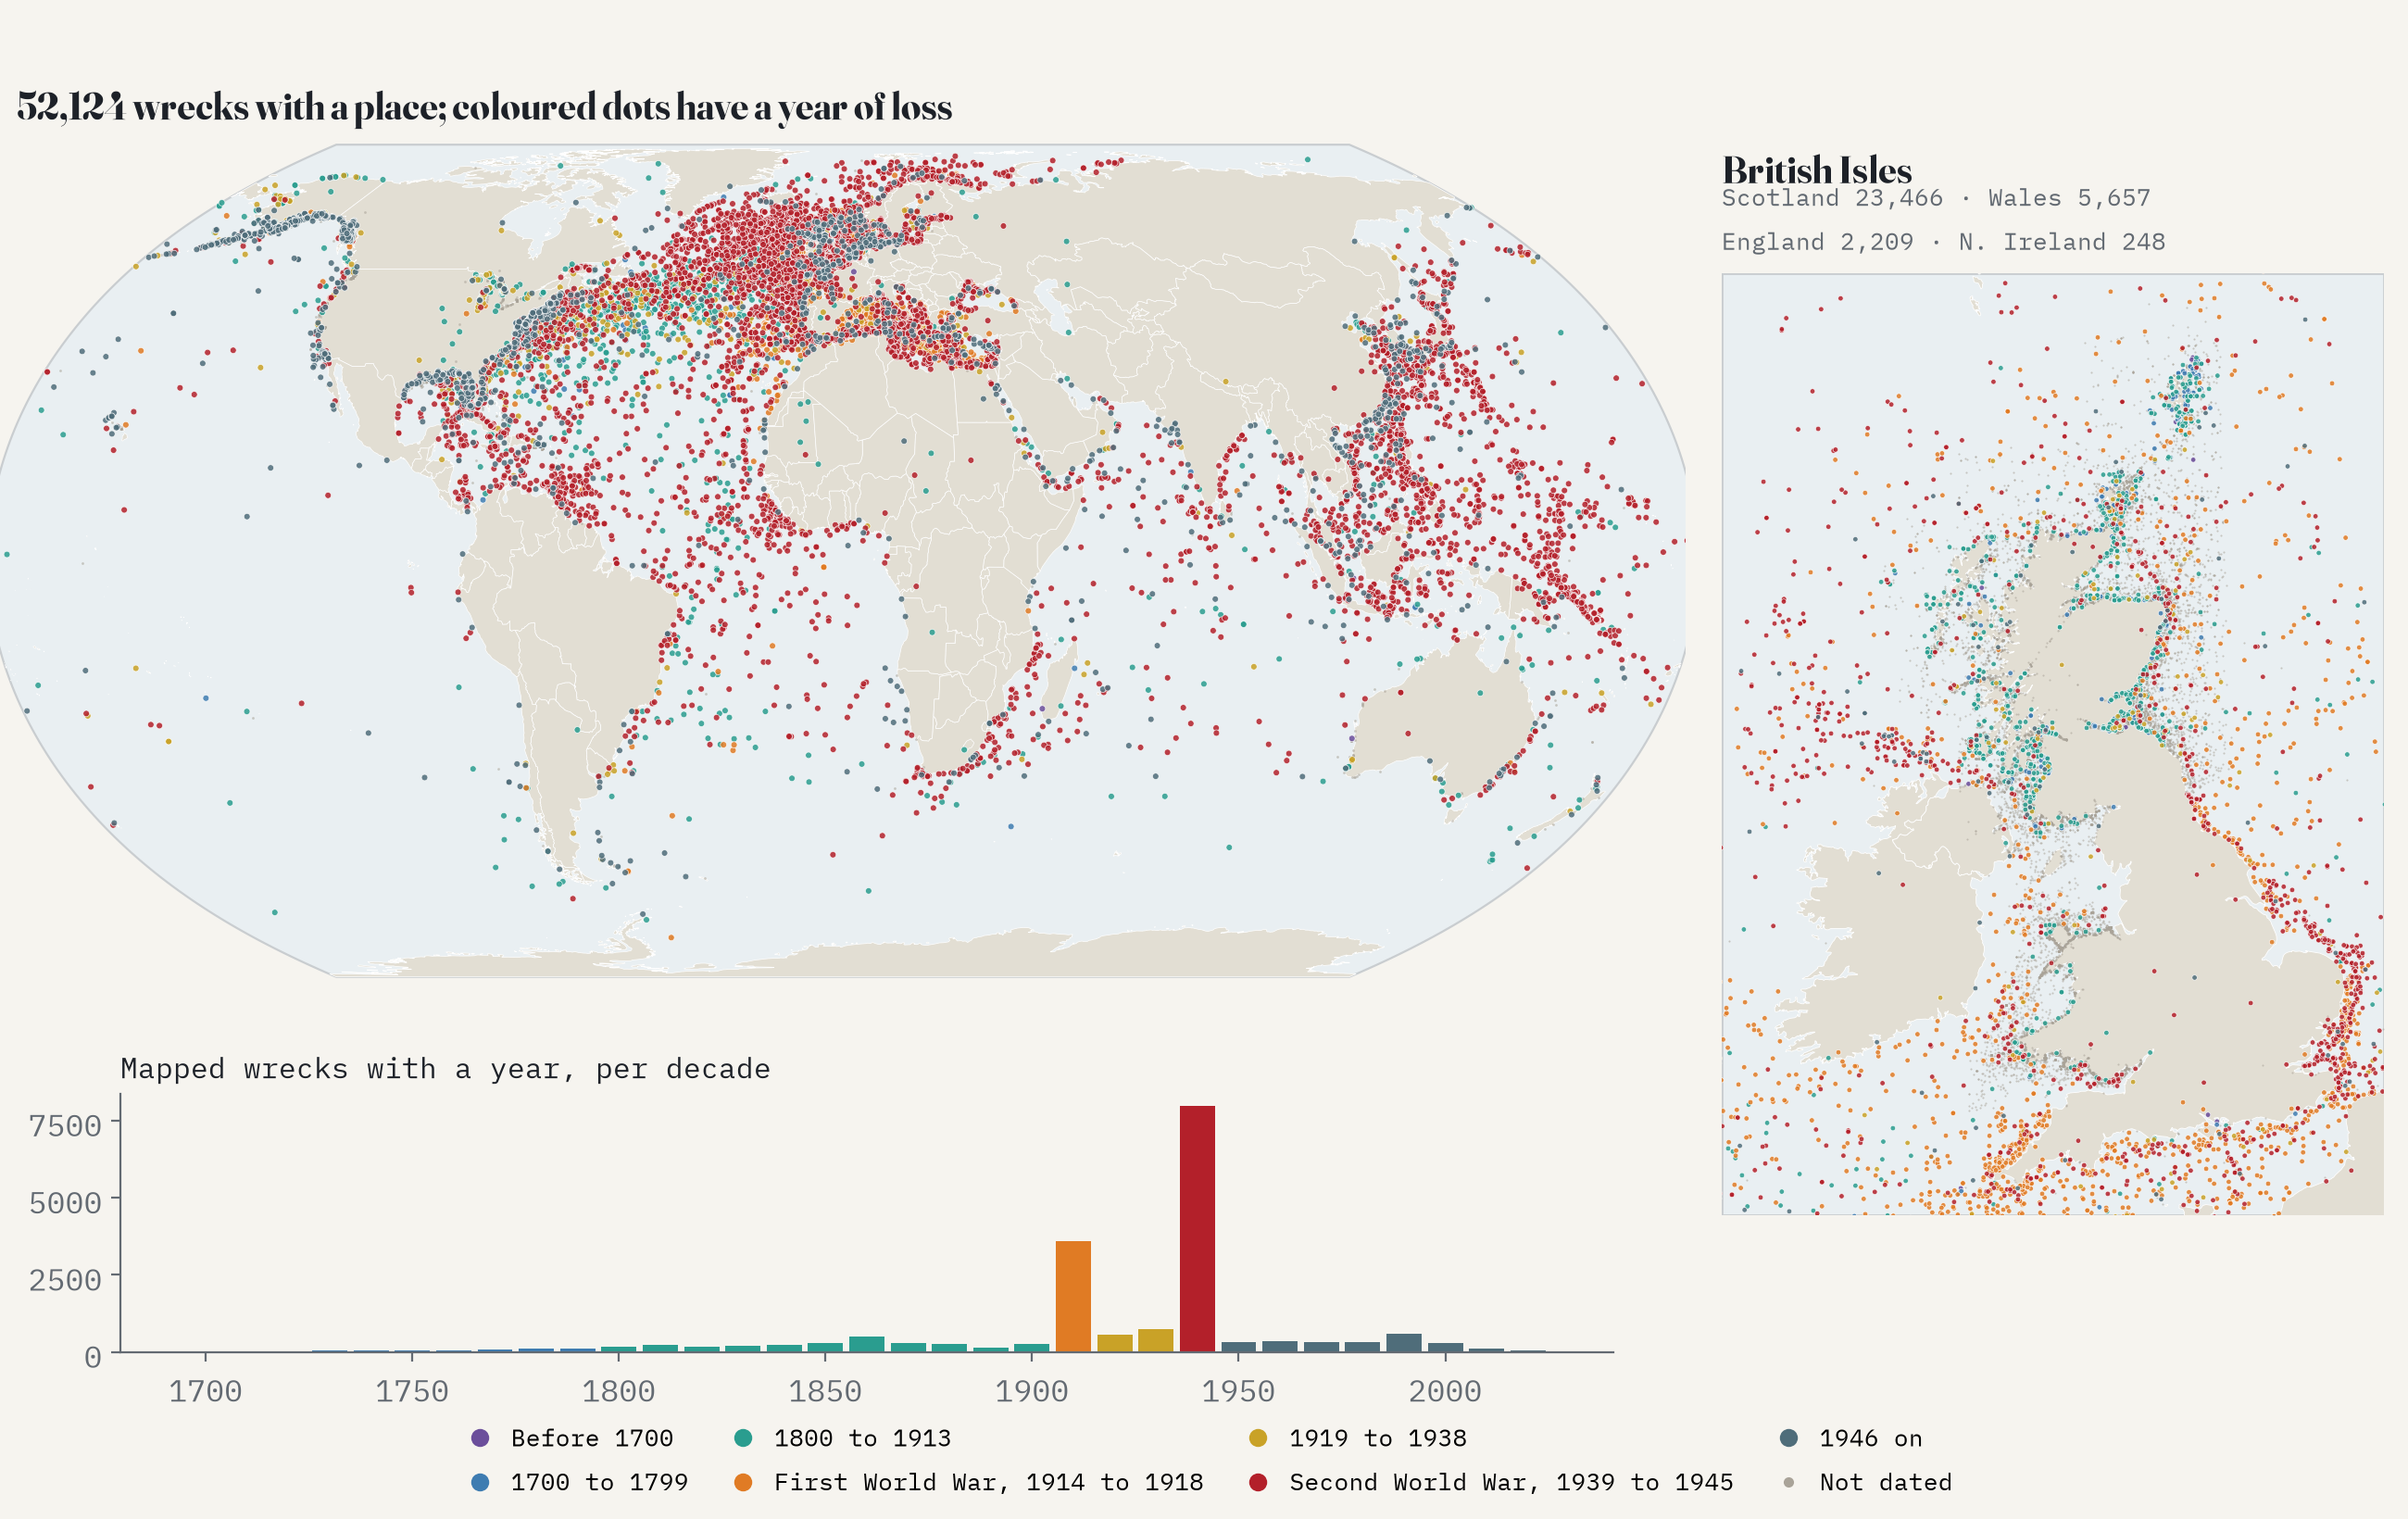
\includegraphics[width=\textwidth]{f_maps.png}
\caption{Mapped wrecks, coloured by era of loss where a year is known (grey: undated), with the British Isles enlarged and mapped wrecks with a year per decade below.}\label{fig:maps}\end{figure}

\begin{figure}[tbp]\centering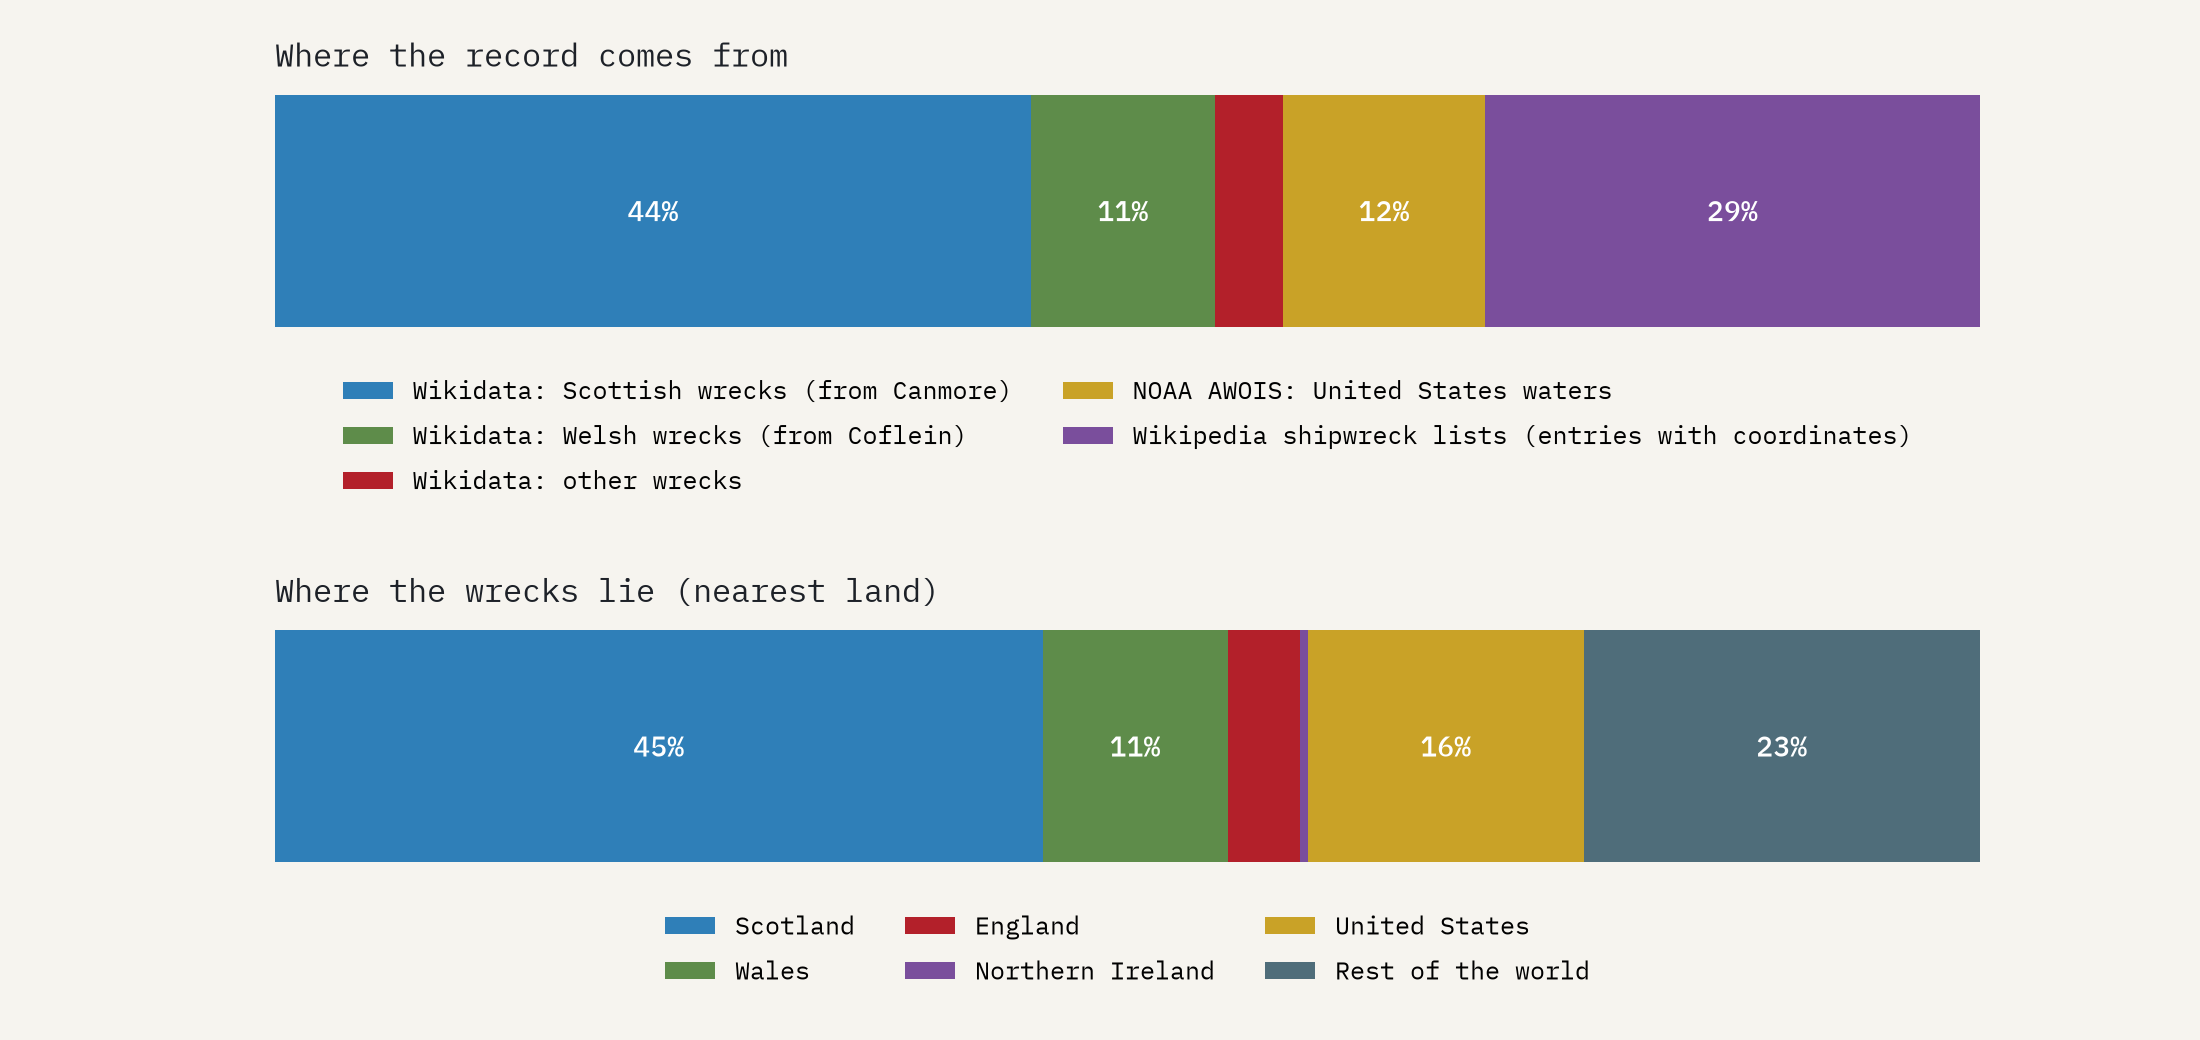
\includegraphics[width=.9\textwidth]{f_record.png}
\caption{Mapped wrecks by source (top) and nearest land (bottom).}\label{fig:record}\end{figure}

\begin{figure}[tbp]\centering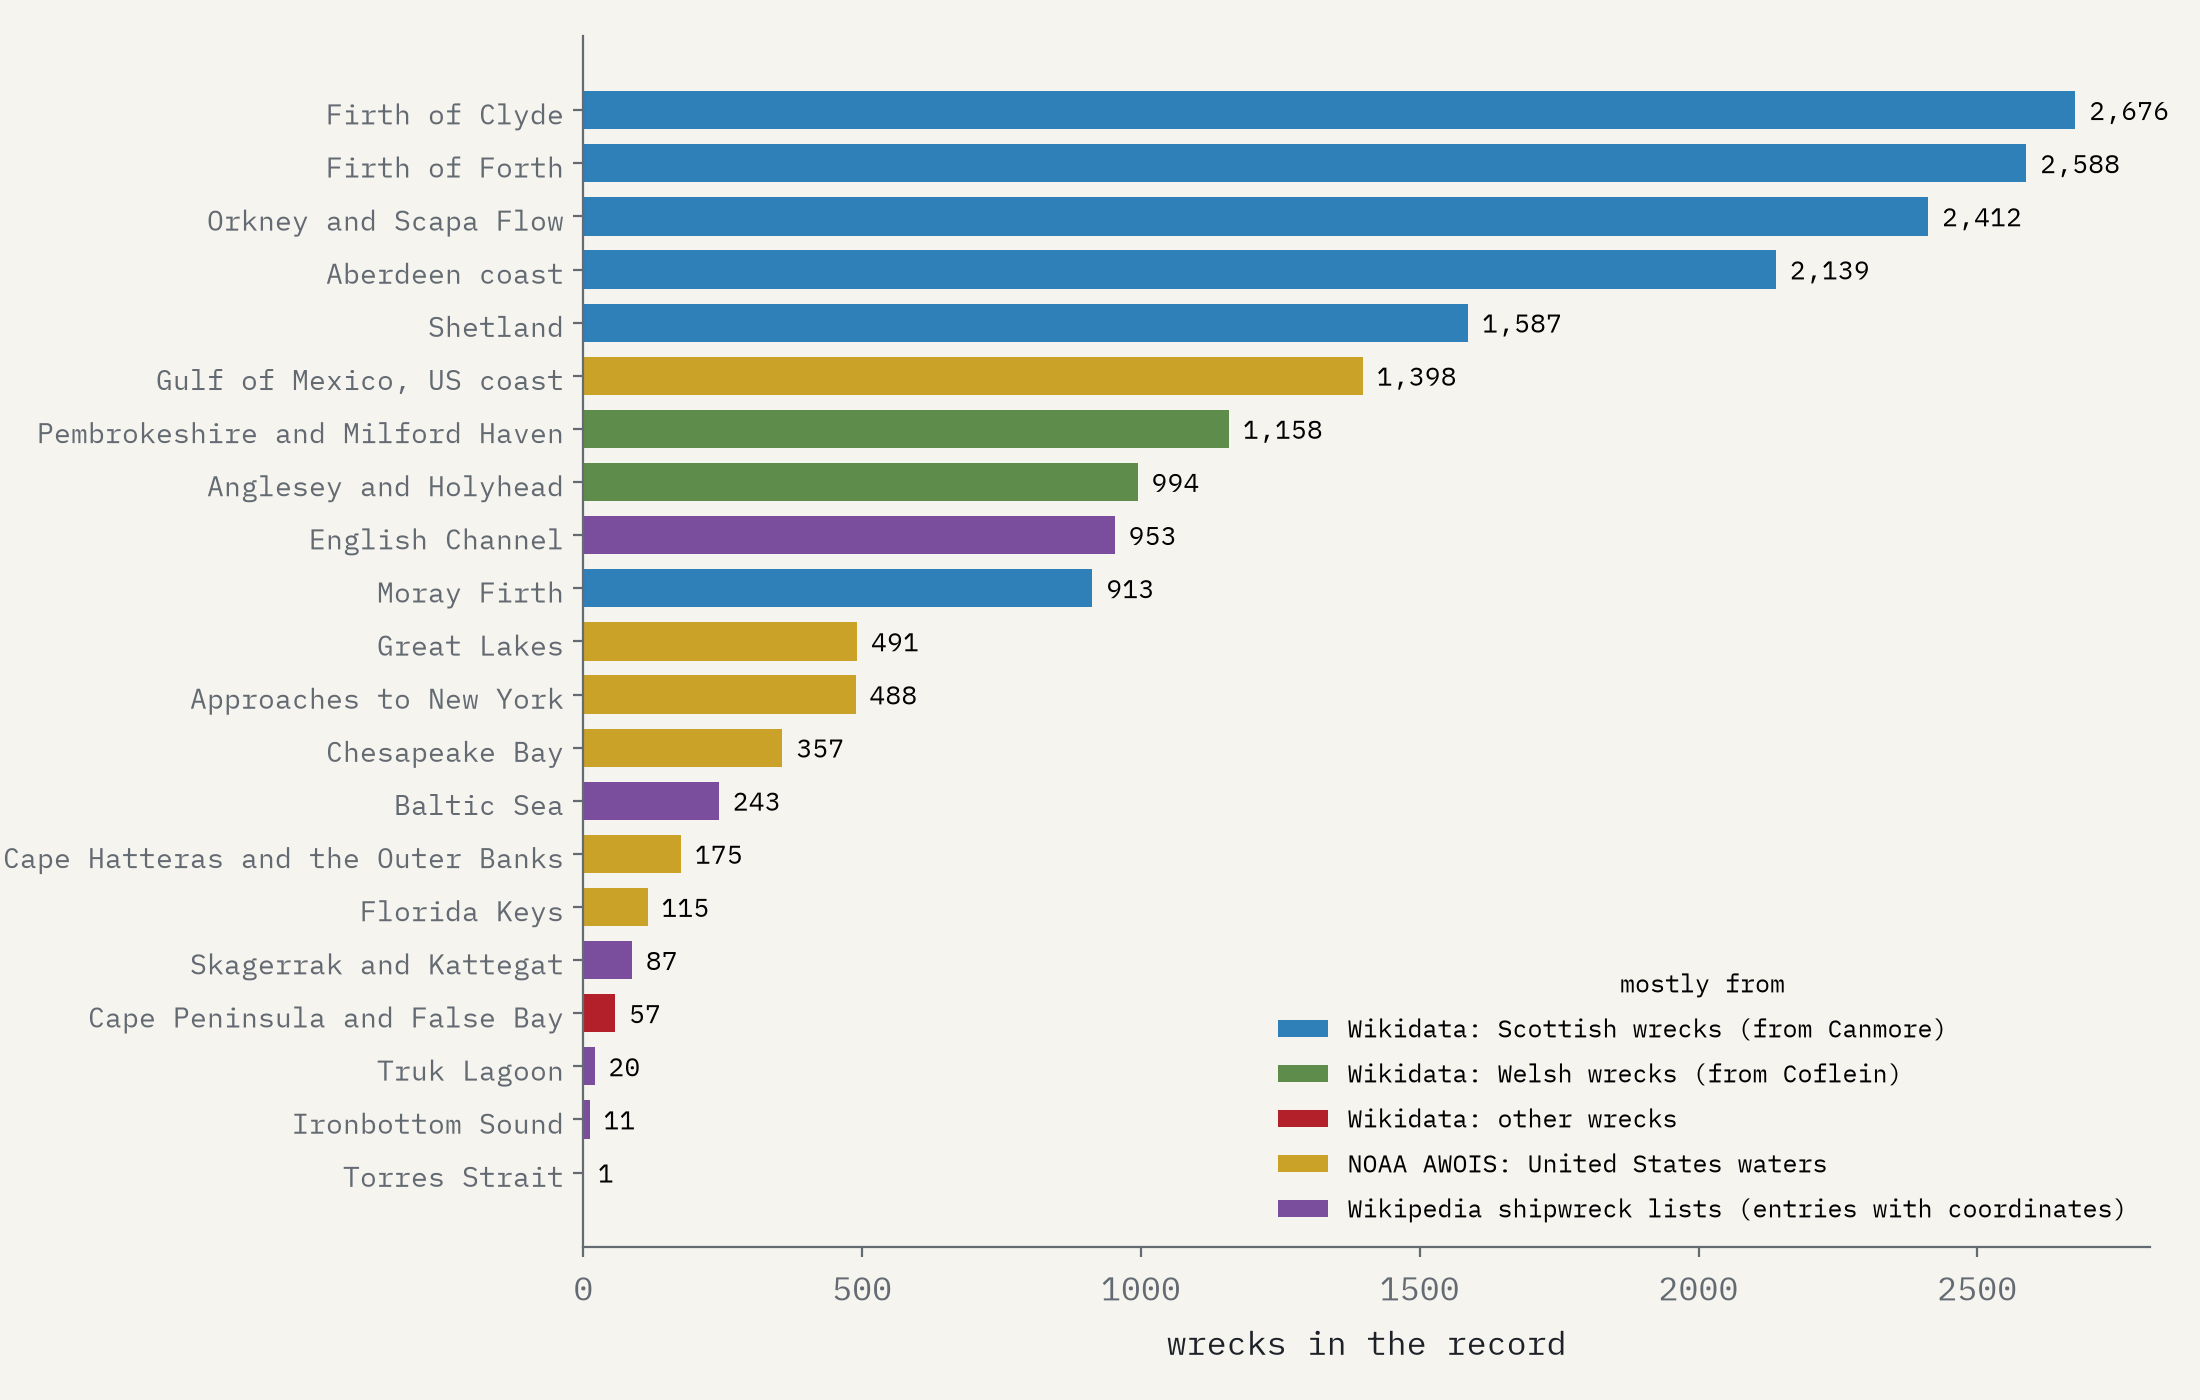
\includegraphics[width=.92\textwidth]{f_graveyards.png}
\caption{Mapped wrecks in named graveyards, coloured by the source most of them come from.}\label{fig:gy}\end{figure}

\begin{table}[tbp]\centering\small\caption{Wrecks in named graveyards (simple boxes). WW: dated to 1914 to 1918 or 1939 to 1945.}\label{tab:gy}\begin{tabular}{llrrr}\toprule Area & Where & Wrecks & Dated & WW\\\midrule
Firth of Clyde & Scotland & 2,676 & 143 & 7\\
Firth of Forth & Scotland & 2,588 & 176 & 11\\
Orkney and Scapa Flow & Scotland & 2,412 & 150 & 24\\
Aberdeen coast & Scotland & 2,139 & 161 & 32\\
Shetland & Scotland & 1,587 & 259 & 15\\
Gulf of Mexico, US coast & United States & 1,398 & 330 & 76\\
Pembrokeshire and Milford Haven & Wales & 1,158 & 46 & 25\\
Anglesey and Holyhead & Wales & 994 & 14 & 5\\
English Channel & England and France & 953 & 851 & 793\\
Moray Firth & Scotland & 913 & 68 & 2\\
Great Lakes & United States and Canada & 491 & 211 & 14\\
Approaches to New York & United States & 488 & 148 & 48\\
Chesapeake Bay & United States & 357 & 48 & 18\\
Baltic Sea & Northern Europe & 243 & 177 & 139\\
Cape Hatteras and the Outer Banks & United States & 175 & 88 & 73\\
Florida Keys & United States & 115 & 36 & 23\\
Skagerrak and Kattegat & Denmark, Norway and Sweden & 87 & 81 & 65\\
Cape Peninsula and False Bay & South Africa & 57 & 7 & 5\\
Truk Lagoon & Micronesia & 20 & 19 & 19\\
Ironbottom Sound & Solomon Islands & 11 & 11 & 11\\
Torres Strait & Australia and Papua New Guinea & 1 & 1 & 0\\
\bottomrule\end{tabular}\end{table}

\subsection{Before 1700}
The oldest dated wrecks in Wikidata are the Dokos wreck (2150~BC), the Uluburun ship (1305~BC) and the Antikythera wreck (61~BC) (Table~\ref{tab:oldest}). The Summary Geodatabase of Shipwrecks gives a fuller view of antiquity (Figure~\ref{fig:ancient}): of its 1,936 wrecks, 1,598 have a date range of 300 years or less, and spreading each over its range the busiest century is the AD 1st century (about 382), the pattern \citet{parker} and \citet{wilson} read as a proxy for Roman trade.

\begin{figure}[tbp]\centering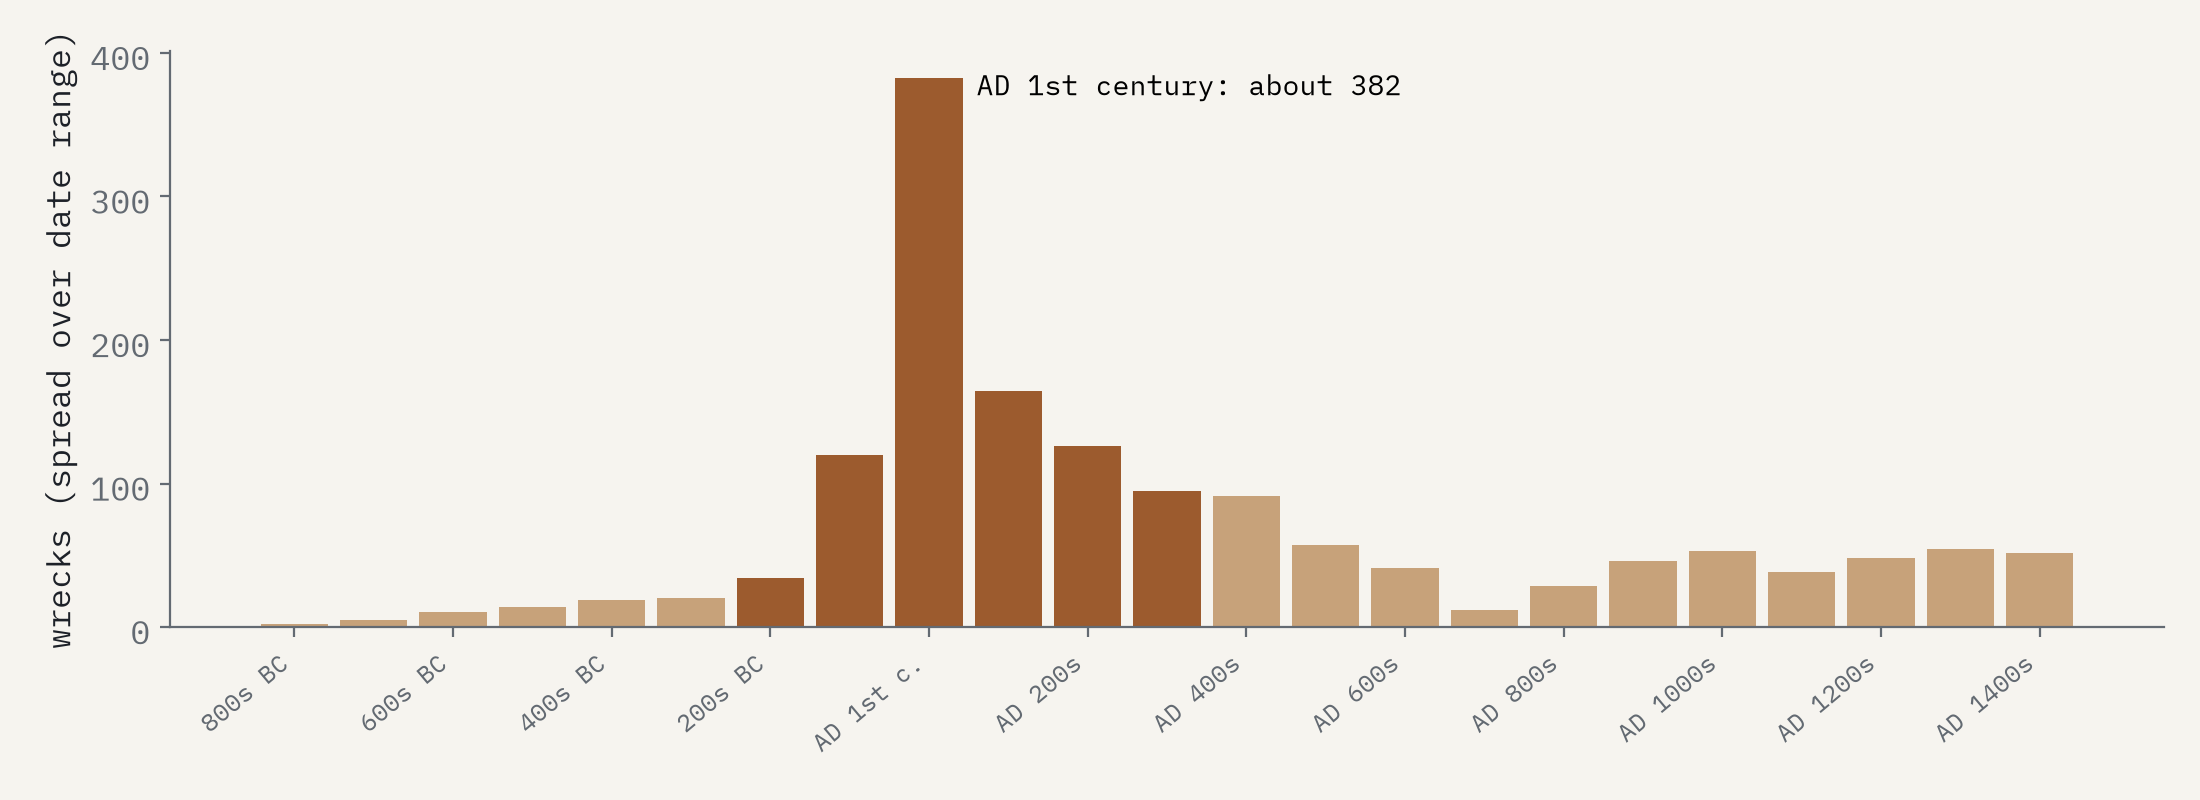
\includegraphics[width=.92\textwidth]{f_ancient.png}
\caption{Wrecks per century in the Summary Geodatabase of Shipwrecks, each spread over its date range. Darker: the Roman era.}\label{fig:ancient}\end{figure}

\begin{table}[tbp]\centering\small\caption{The oldest dated wrecks in the combined record.}\label{tab:oldest}\begin{tabular}{p{4.2cm}rp{3.2cm}p{5.2cm}}\toprule Wreck & Year & Nearest land & Year from\\\midrule
Dokos shipwreck & 2150~BC & Greece & Wikidata: date of the shipwrecking or sinking event\\
Uluburun shipwreck & 1305~BC & Turkey & Wikidata: point in time\\
Bajo de la Campana shipwreck & 701~BC & Spain & Wikidata: inception of a wreck-only item\\
Antikythera wreck & 61~BC & Greece & Wikidata: point in time\\
Belitung shipwreck & 830 & Indonesia & Wikidata: service retirement\\
boat of Barbeau & 1300 & France & Wikidata: inception of a wreck-only item\\
Aber Wrac'h 1 & 1435 & France & Wikidata: date of the shipwrecking or sinking event\\
Grace Dieu & 1439 & England, UK & text: sank or wrecked in a year\\
Iturritxiki & 1520 & Spain & Wikidata: point in time\\
Flor de Rosa & 1528 & Madagascar & Wikidata: date of the shipwrecking or sinking event\\
Mary Rose & 1545 & England, UK & Wikidata: date of the shipwrecking or sinking event\\
Unknown 1548 & 1548 & Scotland, UK & label: unknown vessel lost in a year (Canmore)\\
San Esteban (1554 shipwreck) & 1554 & United States & text: sank or wrecked in a year\\
Mars & 1564 & Sweden & Wikidata: date of the shipwrecking or sinking event\\
\bottomrule\end{tabular}\end{table}

\section{Discussion}
The list series confirms what every maritime historian would expect of the twentieth century: the world wars, and above all the Second, were the most destructive years for shipping on record, and the lists show it even though their coverage of the twentieth century is far thinner than of the nineteenth. The nineteenth-century plateau needs more care. Its height owes much to the sources editors used: digitised British newspapers and Lloyd's List, which reported losses of British-registered and British-insured ships with great regularity \citep{lloyds}. The sharp fall after the 1880s coincides with the end of the newspaper runs most heavily used, not with any sudden change at sea, even if the shift from sail to steam did make shipping safer over the period. Comparisons across periods are therefore unsafe; comparisons of shape within a period, and of causes and flags, are more robust.

\section{Limitations}
First, the series counts entries in a volunteer compilation, not wrecks: coverage varies with sources, editors and decades. Second, it is weighted to British ships and British sources in the 1800s. Third, the scrape buckets causes from short descriptions, and 12\% of entries have none. Fourth, some ships appear in more than one list (for example when damaged and later lost); I removed only exact repeats. Fifth, the map is dominated by the Canmore and Coflein imports and by AWOIS, and only 36\% of mapped wrecks have a year. Sixth, depth is not recorded for most wrecks. Finally, the ancient catalogue is used only in aggregate.

\section{Conclusion}
Wikipedia's shipwreck lists make it possible to count recorded shipwrecks year by year over three centuries. The counts show the world wars standing above everything else, and a long nineteenth-century plateau of strandings and founderings that tells us as much about British newspapers as about the sea. Read with that caveat, they are a remarkable, open, reusable record.

\section*{Data and code availability}
The interactive map is at \url{https://maps.tristanhotham.com/world-shipwrecks/}. Data and code are at \url{https://github.com/Tristan-Hotham/world-shipwrecks} and archived with this paper at https://doi.org/10.5281/zenodo.23850289. The derived Wikipedia list table is released under CC BY-SA 4.0, other derived data under CC BY 4.0, and code under the MIT licence. Wikidata is CC0; AWOIS is a public-domain US Government work; the ancient wreck catalogue is not redistributed.

\section*{AI statement}
I wrote the text, with drafting and editing assistance from Claude (Anthropic), which also helped prepare the analysis code. I reviewed and checked all text and results.

\begin{thebibliography}{9}
\bibitem[AWOIS mirror(2026)]{awoisgh} Bowden, J. A. (2026) AWOIS-data. GitHub repository. \url{https://github.com/jalbertbowden/AWOIS-data}
\bibitem[Canmore(2026)]{canmore} Historic Environment Scotland (2026) Canmore: the national record of the historic environment. \url{https://canmore.org.uk/}
\bibitem[Coflein(2026)]{coflein} Royal Commission on the Ancient and Historical Monuments of Wales (2026) Coflein. \url{https://coflein.gov.uk/}
\bibitem[Lloyd's List(2026)]{lloyds} Lloyd's List (1734 onwards) London: Lloyd's. Shipping news and casualty reports, cited throughout the Wikipedia lists of shipwrecks.
\bibitem[Mangelson(2024)]{ancientgh} Mangelson, A. (2024) ancient\_shipwrecks: Summary Geodatabase of Shipwrecks 1500BCE to 1500CE. GitHub repository. \url{https://github.com/austinw8/ancient_shipwrecks}
\bibitem[Natural Earth(2026)]{naturalearth} Natural Earth (2026) Admin 0 countries, admin 1 units and populated places. Public domain. \url{https://www.naturalearthdata.com/}
\bibitem[NOAA(2026)]{awois} NOAA Office of Coast Survey (2026) Automated Wreck and Obstruction Information System (AWOIS) and Wrecks and Obstructions Database. \url{https://nauticalcharts.noaa.gov/data/wrecks-and-obstructions.html}
\bibitem[Parker(1992)]{parker} Parker, A. J. (1992) \emph{Ancient Shipwrecks of the Mediterranean and the Roman Provinces}. Oxford: BAR International Series 580.
\bibitem[Strauss(2013)]{strauss} Strauss, J. (2013) Shipwrecks Database. Version 1.0. Oxford Roman Economy Project. \url{http://oxrep.classics.ox.ac.uk/databases/shipwrecks_database/}
\bibitem[UNESCO(2026)]{unesco} UNESCO (2026) Underwater cultural heritage. \url{https://www.unesco.org/en/underwater-heritage}
\bibitem[Wikipedia(2026)]{wikilists} Wikipedia contributors (2026) Lists of shipwrecks (List of shipwrecks in \emph{month year}, 1700 to 2025). CC BY-SA 4.0. \url{https://en.wikipedia.org/wiki/Lists_of_shipwrecks}
\bibitem[Wikidata(2026)]{wikidata} Wikidata (2026) Wikidata, the free knowledge base. CC0. \url{https://www.wikidata.org/}, queried with QLever, \url{https://qlever.cs.uni-freiburg.de/}
\bibitem[Wilson(2011)]{wilson} Wilson, A. (2011) Developments in Mediterranean shipping and maritime trade from the Hellenistic period to AD 1000. In Robinson, D. and Wilson, A. (eds) \emph{Maritime Archaeology and Ancient Trade in the Mediterranean}. Oxford: Oxford Centre for Maritime Archaeology, 33 to 59.
\end{thebibliography}
\end{document}
